%%%%%%%%%%%%%%%%%%%%%%%%%%%%%%%% 
\section{The Field Cage and High Voltage System} 
\label{sec:detectors-fd-alt-hv}

A detailed description of the design of the HV system, field cage and cathode for the LBNO 20kton and 50 kton detectors is provided in the deliverable document 3.1 (LAr experiment) of the LAGUNA-LBNO design study \cite{LAGUNA-LBNO-deliv}. This design can be applied to the DUNE 12kton or 15kton detectors with some simplifications and down-sizing due to the shorter drift path and the rectangular aspect ratio of the detector. The much shorter transversal dimension with respect to LBNO allows to construct a lighter cathode structure (less sagging effect to be compensated with respect to the octagonal detector) and to simplify the hanging system of the drift cage and the cathode.

The field cage in the LAGUNA-LBNO double-phase detector design  is composed of equally spaced octagonal rings which create a uniform drift field with strength between 500 and 1000 V/cm. A  voltage up to 2 MV at the cathode is then needed in order to provide a the drift field at the maximal intensity of 1 kV/cm over a drift distance of 20 m.

Two different approaches have been considered and realized for the drift field HV system. The first type uses an external HV power supply and feeds it into the detector volume using HV feedthroughs. This approach is going to be applied in the WA105 demonstrator for a drift of 6m and a cathode voltage up to 600 kV.  The second approach is based on an internal HV generator directly inside the LAr volume same as the Greinacher HV multiplier. It is an innovative technique to generate a HV for creating a drift electric field in a LAr-TPC, with some advantages compared to the first option. This technique particularly suits giant-scale detectors, where a very HV of ~1 MV to ~2 MV is needed. For the DUNE detector (12 m drift) a voltage of 600 kV will be needed in order to operate at a field intensity of 0.5 kV/cm. This voltage is a factor 3.3 higher than the one foreseen in the reference design and it is in the scope of the WA105 detector operation at 1 kV/cm over 6 m drift.

The field cage designed for the LBNO 20 kton detector (20 m drift path) is composed of 99 octagonal field shaping coils manufactured from 316L stainless steel tubing and long radius elbows to EN 10217-7 shop using a combination of welded and clamped joints. Each field shaping coil is designed as a series of fully welded infill tubes to fit between hanging columns to form one section of the field cage. The coils are then supported by 32 off hanging columns suspended from the tank deck structure by a special hanging support system. The design foresees hanging columns built in the form of chains. Short sections of the field shaping coils are integrated as pins into links of G-10CR glass fibre/epoxy laminated sheet insulating material to assemble each one of these chains. Longer sections and corner sections of the field shaping coil are then fixed in between the hanging columns to complete each coil (Figure~\ref{fig:LBNO_FC}). The combined assembly of 99 sets of field shaping coils within the 32 off hanging columns thus provides a complete field cage.

\begin{cdrfigure}[Assembly concept of the field cage]{LBNO_FC}{\small Left: assembly of the elements of a hanging chain. Right: construction of a field cage section from the hanging chains and the field shaping coil elements.}
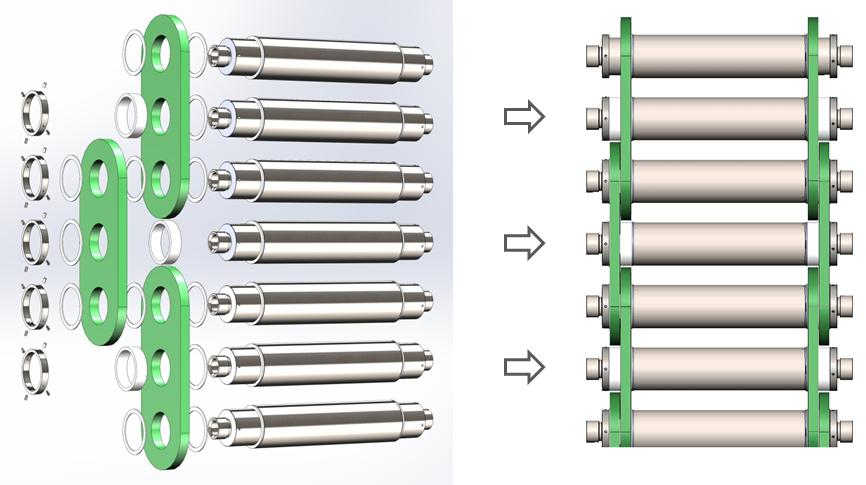
\includegraphics[width=.5\linewidth]{LBNO_chains} \hfill
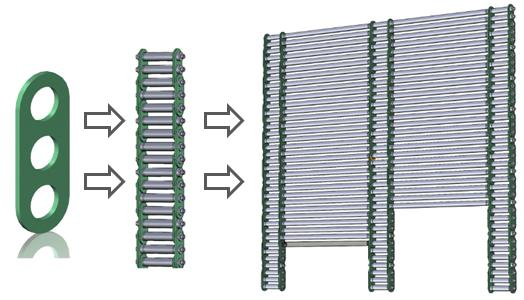
\includegraphics[width=.4\linewidth]{LBNO_FC2}
\end{cdrfigure}

The tubes specifications foresee an outer diameter of  139.7 mm which is common to the cathode structure but allow a thinner wall section to be used where required in a non-structural parts pf the field shaping coils.  Although a non-standard size, the total length of 1.6mm wall thickness tube required for the field shaping coils can be manufactured as a special mill run.  Using this approach it will be possible to save 21 tons of material as compared with the standard 2.0mm wall thickness of the tubes. The link pins have 2.6 mm wall thickness. This will provide sufficient section modulus to react the bending moments across the link pins. All specialist preparation and welding of the link pins will be carried out under controlled fabrication shop facilities.  This will comprise the rough machining of the end fittings, preparation of the tube ends and the jig welding of the complete assemblies. Further machining, after welding will be carried out to ensure correct alignment and tolerance levels in conjunction with the hanging columns.  Vent holes will be incorporated into the tubes as required to facilitate construction and to allow purging with GAr/LAr on commissioning.

A fundamental part of the field shaping coil design process, in collaboration with the LAGUNA-LBNO industrial partners, involved the consideration of how such tubes could be manufactured to a high level of accuracy, transported to site, moved underground and then constructed in a 'Clean Room' environment within the completed membrane tank.  This requirement presented considerable challenges in terms of logistics and the development of the overall concept for fabrication.  It was concluded that a modular construction approach would be required in order to maximize off-site shop fabrication and minimize on-site assembly.  This approach was also considered essential in order to ensure the cleanliness of construction and to minimize the installation time. The breakdown of each field shaping coil is made into sets of 3 main modules.  Although separate modules, the field shaping coils and the cathode structure share identical features and dimensions.  Thus, the maintenance of common interfaces forms an essential part of the overall detector design. The field cage design for the DUNE far detector is based on the same concept developed for LBNO, including 60 rectangular rings used to cover the 12 m of drift volume of the 12 kton detector.

The cathode design for LBNO was developed following an extensive review of options and analysis to optimize the design for the specific requirements of the 50 kton LAr Detector.  The design incorporates features to minimize the static deflection of the cathode and to maximize the electrostatic performance (avoid regions with high electric fields, maximum allowed electric field limited to 50 kV/cm). Also the cathode is designed in a modular structure for maximum off-site shop fabrication and minimum on-site assembly in order the ensure cleanliness of construction, by using the cryostat ad clean room for the assembly, and to minimize the installation time. The cathode is designed as a fully welded tubular rectangular (square) grid structure in 2m x 2m bays, 1m deep supported only from the outer periphery (Figure~\ref{fig:LBNO_cathode}).  The top and bottom grid structures are manufactured from 139.7mm OD x 2.6mm wall tubes to EN 10217-7 in 316 stainless steel.  The bracing structure is manufactured from 60.3mm OD x 2.6mm wall tubes also to EN 10217-7 in 316 stainless steel.  A grid structure comprising 10mm OD x 1mm wall tubes arranged in a parallel single plane at 100mm centers will be fitted to the top of the cathode only. The maximum module size is the 6m module comprising 3 full $2m \times 2m \times 1m$ deep bays of the cathode structure.  All specialist node preparation and welding of the modules will be carried out under controlled fabrication shop facilities.  Vent holes are incorporated into the structures to facilitate construction and to allow purging with GAr/LAr on commissioning. High levels of quality control will be possible with the modular construction design and following inspection, each module will be cleaned to ISO 8 cleanliness standard and double wrapped prior to dispatch and transportation to site for installation and final assembly of the cathode. The complete assembly procedure logistics and tooling for the field cage and cathode is described in details the LAGUNA-LBNO deliverable document.

The cathode outer top tubular structure is identical to the bottom field shaping coil  by using tubes with  the same outer diameter (139.7mm).  The spans are the same (48m for the 50 kton LBNO detector) and the vertical distance separating these components is the same as the remaining field shaping coils (200mm centers). The cathode will be attached at the bottom of each hanging column by a split link in G-10CR. , The cathode attachment points will also incorporate locally thickened sections of tube (as in the hanging chains) included as part of the peripheral structure nodes


The cathode structure for the 12 kton DUNE far detector follows the same design concepts as the one studied for LBNO with a down-sizing of the elements since is is not needed to limit sagging effects over 48 m span but on only 12 m. This translates in a lighter and cheaper structure. 

\begin{cdrfigure}[Cathode design]{LBNO_cathode}{\small Left: cathode plane design for the LBNO detector. Right: breakdown of the cathode structure in construction modules.}
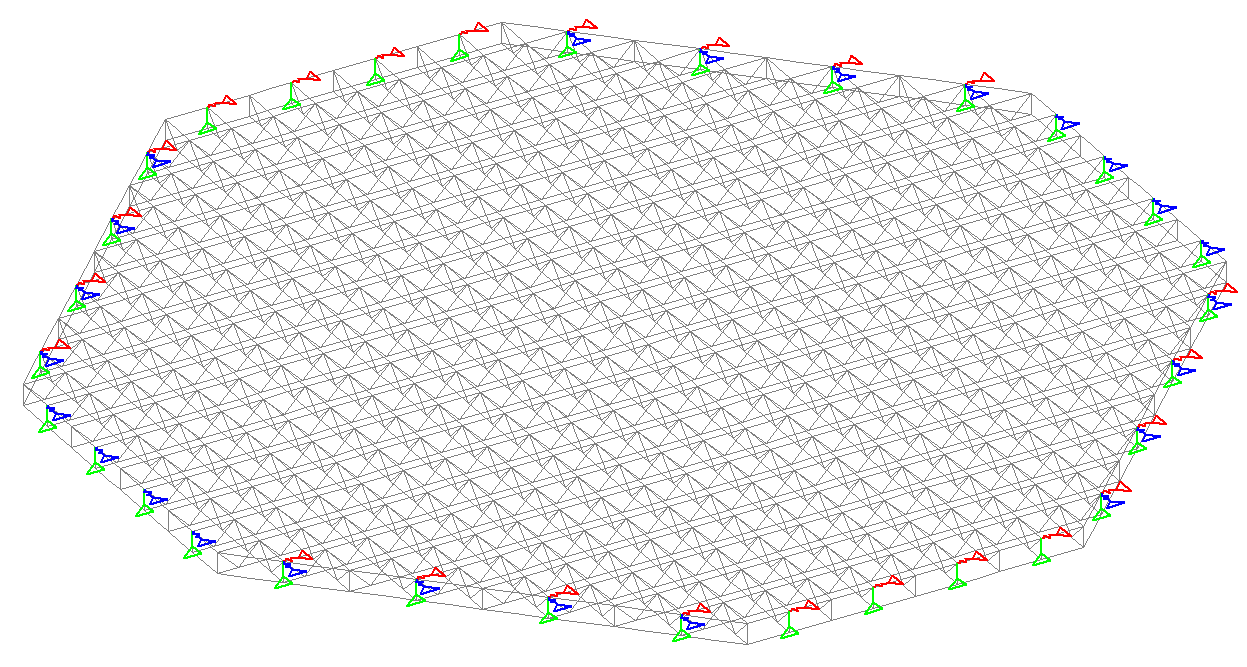
\includegraphics[width=.4\linewidth]{LBNO_cathode} \hfil
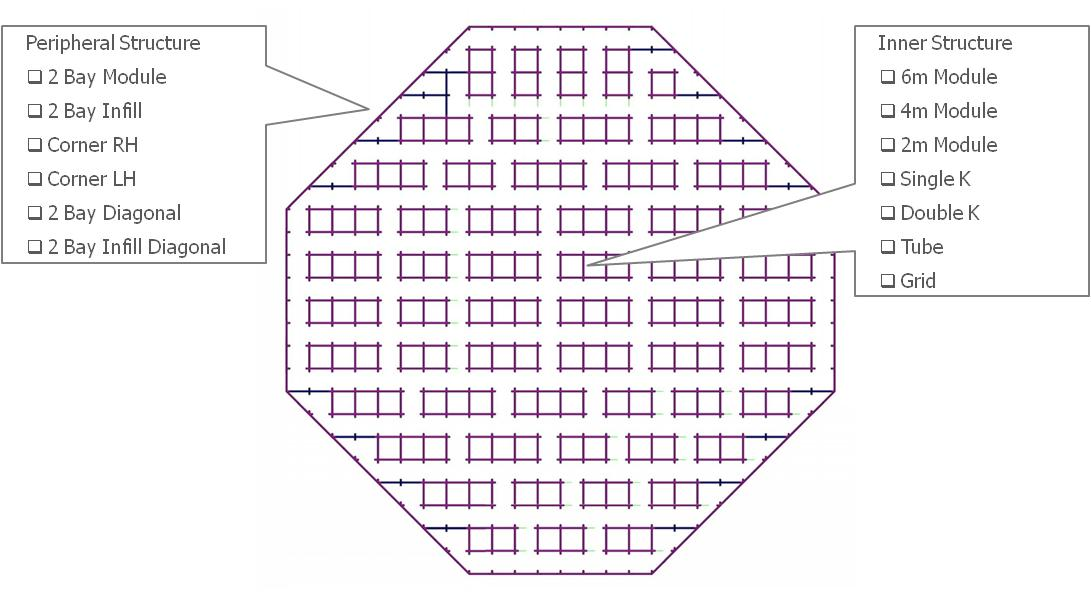
\includegraphics[width=.5\linewidth]{LBNO_cathode_elements}
\end{cdrfigure}


